% !TEX root = ../my-thesis.tex
%

\chapter{Contexte scientifique}
\label{sec:contexte}

\cleanchapterquote{Un petit chapitre pour le doctorant, un grand chapitre pour l'humanité}{Doctorant anonyme}{(Citation temporaire)}


\section{Contexte clinique}
\label{sec:contexte:clinique}

Le foie est un organe vital pour le fonctionnement du corps humain. Il est impliqué dans de nombreux systèmes vitaux : contrôle de la glycémie, élimination des toxines du sang, participation à la digestion et au système immunitaire. Le suivi des dysfonctionnements de cet organe est donc crucial pour les médecins.

Le foie est situé au niveau de l'abdomen, au-dessous des poumons. Il est adjacent à l'estomac et au cœur comme illustré dans la figure \ref{fig:liver}.

Dans un système vasculaire classique, le sang oxygéné est apporté par les artères dans les organes. Il passe ensuite à travers un réseau de capillaires dans l'organe au niveau desquels s'effectuent les échanges entre les cellules de l'organe et le sang. Le sang appauvri est ensuite renvoyé vers le cœur par le système veineux. Pour le foie, ce circuit est formé par l'artère hépatique et la veine cave. La particularité du foie est qu'il est alimenté par un second système veineux qui connecte le foie à 3 organes : l'estomac, le pancréas et la rate. C'est par ce système veineux, la veine porte, qu'est alimenté le foie en nutriments.  


\begin{figure}
    \centering
    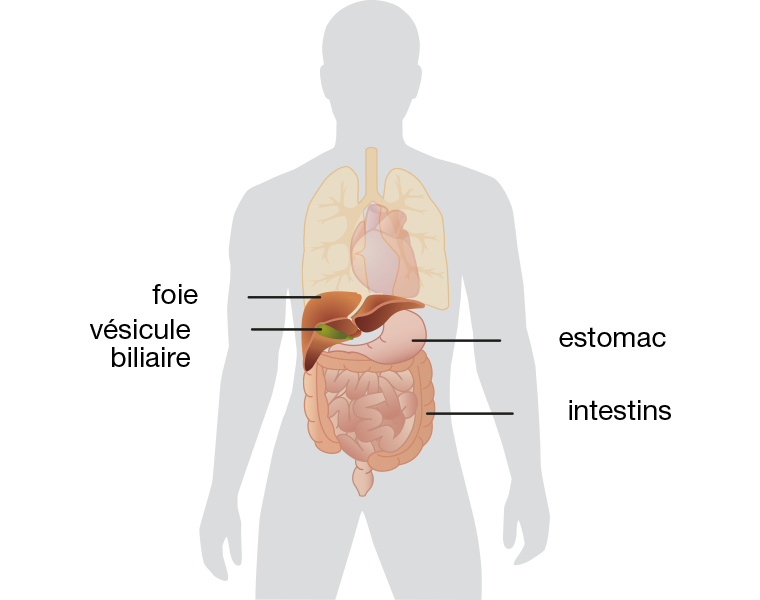
\includegraphics[height=6cm]{Images/Liver.png}
    \caption{Foie humain.}
    \label{fig:liver}
\end{figure}

La veine cave est connectée au foie par sa partie supérieure alors que la veine porte entre dans le foie par son centre via le tronc porte. Le tronc porte se divise une première fois à l'entrée du foie pour former les veines  porte droite et gauche. Ces deux branches se subdivisent ensuite à plusieurs reprises afin d'alimenter l'ensemble des tissues du foie. 

Un intérêt particulier est attribué à la veine porte puisque ses ramifications forment 6 régions du foie indépendamment approvisionnées les unes des autres. Cette cartographie, illustrée en figure \ref{fig:liver veins} est largement adoptée par les médecins sous le nom de schéma de Couinaud. Ce schéma est utilisé lors de la planification d'opérations d'extraction de tumeurs pour définir les limites des zones à extraire.

\begin{figure}
    \centering
    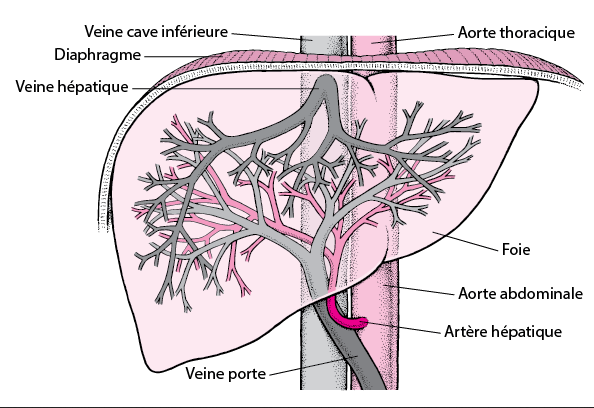
\includegraphics[height=4cm]{Images/Liver_vasculature.png}
    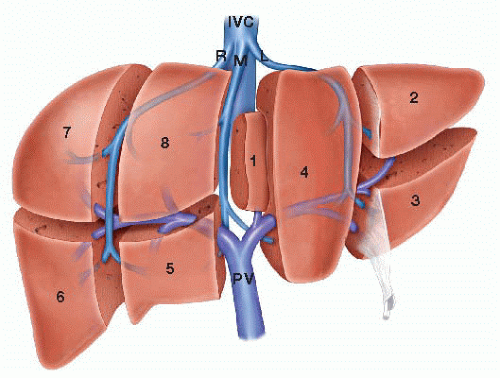
\includegraphics[height=4cm]{Images/Couinaud.png}
    \caption{À gauche, système vasculaire hépatique. À droite, la segmentation de Couinaud.}
    \label{fig:liver veins}
\end{figure}


La hiérarchie des systèmes veineux et artériel est relativement stable dans la population, mais des variations entre les individus peuvent survenir de manière assez fréquente. Une étude, réalisée par Fang et al. \cite{Fang2012_Liver_vein_variations} effectuée sur 200 patients, montre que le schéma "classique" ne représente que 61 \percent des cas. Les 39 \percent restant se divisent en divers cas particuliers. Le réseau lymphatique est aussi présent au niveau du foie, mais leur diamètre réduit rend ce système invisible sur la plupart des imageries hépatiques. Le reste du foie présente un tissu relativement homogène lorsque celui-ci est sain.
Lorsque le foie est malade, l'apparence des systèmes veineux et artériel peut-être extrêmement altérée. 

L'aspect du foie est aussi variable selon son état. Lorsque le foie est atteint de tumeurs, des zones de densités différentes sont visibles et celles-ci peuvent venir altérer les tissus alentours. Pour des maladies comme la cirrhose (voir Fig. \ref{fig:unhealthy liver}), le foie peut changer drastiquement d'aspect et se contracter, réduisant ainsi sa taille et écrasant les vaisseaux. Ceux-ci peuvent ainsi ne plus être détectés lors de l'acquisition d'images. 

\begin{figure}
    \centering
    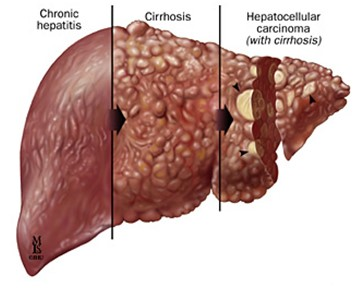
\includegraphics[height=4cm]{Images/Liver_cirrhosis_stages.jpg}
    \caption{Différents stades de maladie du foie.}
    \label{fig:unhealthy liver}
\end{figure}


La plupart des images de foie disponibles sont des images de foie malades dans la mesure où les actes médicaux ne sont pas réalisés sans suspicion de maladie.
\todo{Parmi les recommandations de la haute autorité de santé ?}

\section{Contexte d'acquisition d'images}
\label{sec:contexte:images}

Les avancées technologiques dans l'imagerie médicale sont motivées par le besoin de connaitre le corps du patient tout en limitant les opérations intrusives. Des techniques permettant d'obtenir une image d'une partie interne du corps ou d'un organe ont donc vu le jour. On peut par exemple citer l'imagerie par ultrason qui permet d'obtenir une image en envoyant des ondes sonores à travers un medium. Le calcul du temps de propagation permet ensuite de générer une image en fonction de la densité des tissus traversés. On peut aussi citer la plaque radiographique, qui permet de créer une image en deux dimensions en exposant une plaque sensible aux rayonnements à une source de photons. En plaçant le corps entre la plaque et la source, les tissus filtrent une partie des faisceaux qui atteignent la plaque, permettant de voir à travers les tissus de faible densité. Des exemples de ces deux techniques sont montrés en Fig. \ref{fig:2D imaging}.

\begin{figure}
    \centering
    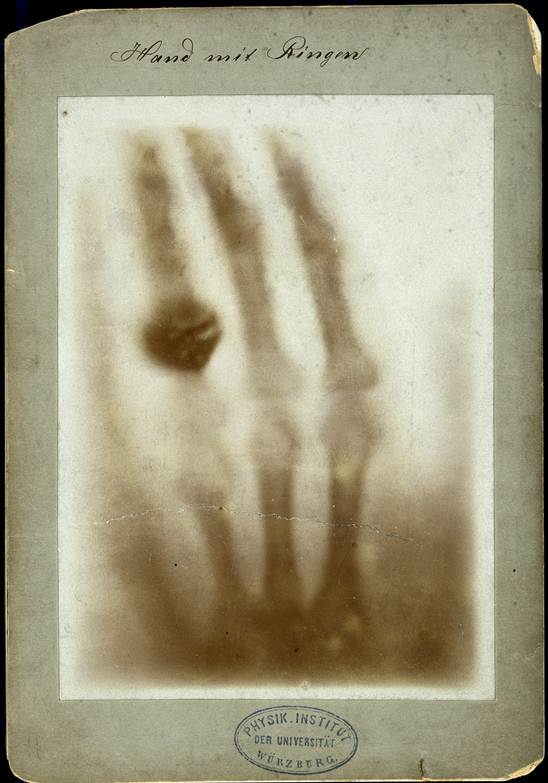
\includegraphics[height=4cm]{Images/first_CT.png}
    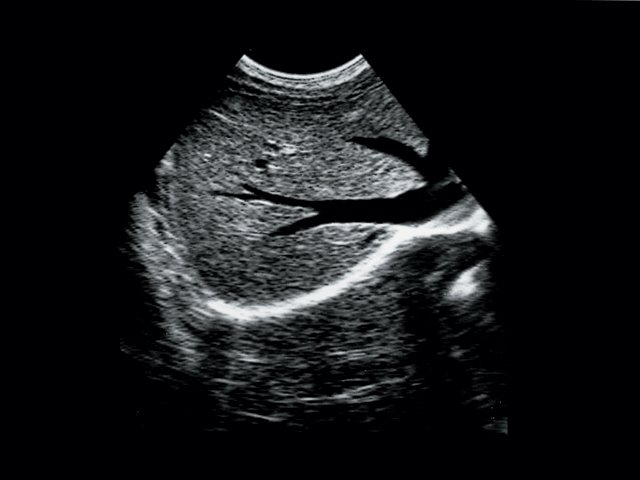
\includegraphics[height=4cm]{Images/Liver_ultrasound.jpg}
    \caption{Exemples d'acquisitions 2D : À gauche, la première image obtenue par rayons X (Roentgen, 1895). À Droite, Image par ultrason du foie. La veine porte est visible en noir.}
    \label{fig:2D imaging}
\end{figure}

Ces méthodes, à l'origine limitées à la 2D, ne permettaient pas d'avoir un rendu des organes en trois dimensions. Deux techniques, communément employées, aujourd'hui ont donc été développées pour acquérir des images volumiques.

\subsection{Tomodensitométrie}
\label{sec:contexte:images:CT}

La tomodensitométrie (TDM) est un système reposant sur l'émission de rayons X développée en 1979 par Houndfield et al. \cite{Houndfield1995_CT_machine}.

Le patient est allongé sur une table autour de laquelle est positionné un anneau. La table du patient est déplacée dans l'axe des pieds à la tête (axe longitudinal). L'anneau de la machine tomodensitométrique contient un tube émetteur de rayons X ainsi qu'une rangée de détecteurs sur la partie opposée de l'anneau. L'anneau tourne autour du patient afin d'acquérir le plan XY, ou plan axial. Pour les acquisitions avec une table immobile, on parle de mode axial ou séquentiel. Lorsque la table est en mouvement pendant l'acquisition, on parle de mode spiralé ou hélicoïdal. Cette technologie est irradiante, car une image est obtenue grâce à l'absorption du rayonnement par les organes qui atténuent de fait le signal reçu par les capteurs.  Une exposition à un rayonnement important peut être à l'origine de cancers, c'est pourquoi les doses auxquelles sont exposés les patients sont très contrôlées par les radiologues.

Les images produites par un système CT sont des sinogrammes, un type d'images qui contient la projection du profil détecté pour un certain angle du capteur. Chaque ligne du sinogramme représente ainsi la projection pour un angle donné. On peut ensuite reconstituer une image 2D grâce à la transformée de Radon (plus précisément son inverse), qui permet de reconstituer un point dans l'espace à partir de la totalité de ses projections. L'ensemble du processus est illustré en Fig. \ref{fig:tomography}.

\begin{figure}
    \centering
    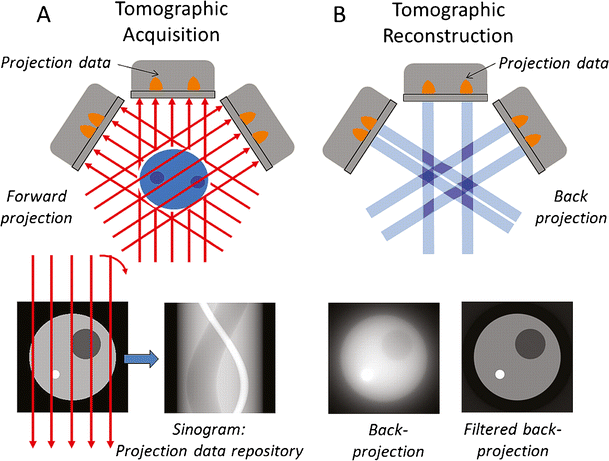
\includegraphics[height=6cm]{Images/Tomo_projection.png}
    \caption{Acquisition par projection et reconstruction du signal. La reconstruction étant finie, des artefacts de flou peuvent être présent.}
    \label{fig:tomography}
\end{figure}

\subsubsection{Artefacts des images Tomodensitométriques}

Les artefacts liés à la tomodensitométrie sont multiples. Premièrement, la qualité de l'image dépend du nombre de projections disponibles. Les structures peuvent être floues du fait de la reconstruction. En effet, en théorie une image nette est obtenue par la reconstruction d'un nombre infini de projections. En pratique le nombre de projections est défini et choisi comme un compromis entre rapidité d'acquisition et qualité de l'image. Le flou peut avoir d'autres causes telles que les mouvements du patient, la distance à la source, où être causé par l'absorption des tissus. 

\begin{figure}
    \centering
    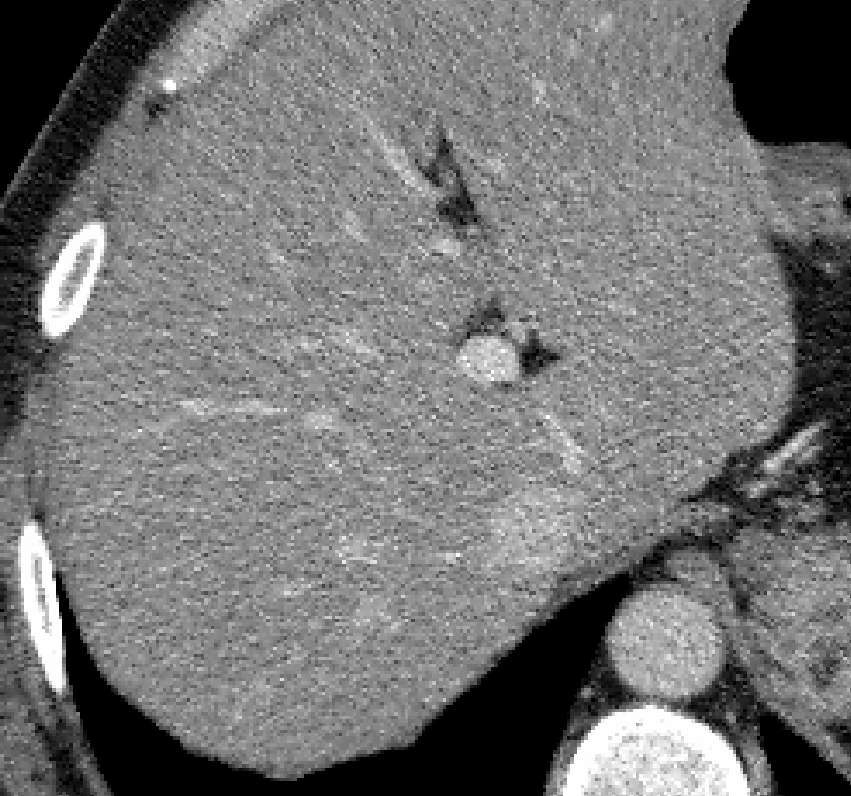
\includegraphics[height=4cm]{Images/blury_vessels.png}
    \caption{Coupe d'une tomographie du foie. Les taches floues et claires  correspondent aux vaisseaux hépatiques}
    \label{fig:CT_blur}
\end{figure}

\todo{@Bertrand: Je suis pas sûr de voir l’aspect « aléatoire » dans l’émission ?}
\todoNote{https://www.ncbi.nlm.nih.gov/pmc/articles/PMC2579780/}
\todoNote{While the noise propagation through detection and calibration operations is a complicated process, the noise distribution at the X-ray generation stage can be expressed as a Poisson functional (Macovski 1982). }

Deuxièmement, les images tomodensitométriques montrent toutes un profil bruité (Fig. \ref{fig:CT_noise}). Ce bruit est issu de la source de photon qui les émet de manière aléatoire. En théorie ce phénomène suit une loi de probabilité de Poisson. Cependant, le bruit affectant les images à la fin du processus est un bruit additif blanc gaussien \cite{Lei1992_gaussianNoiseCT}. Ce bruit est défini par la densité de probabilité suivante :

\begin{equation}
\frac{1}{\pi \sqrt{2\pi} } exp\big( \frac{ (x-\mu)^2}{2\sigma^2} )    
\end{equation}

Cette densité est paramétrée par l'intensité moyenne du bruit $\mu$ et son écart-type $\sigma$ qui correspond à la dispersion des valeurs d'intensité du bruit autour de sa moyenne.

\begin{figure}
    \centering
    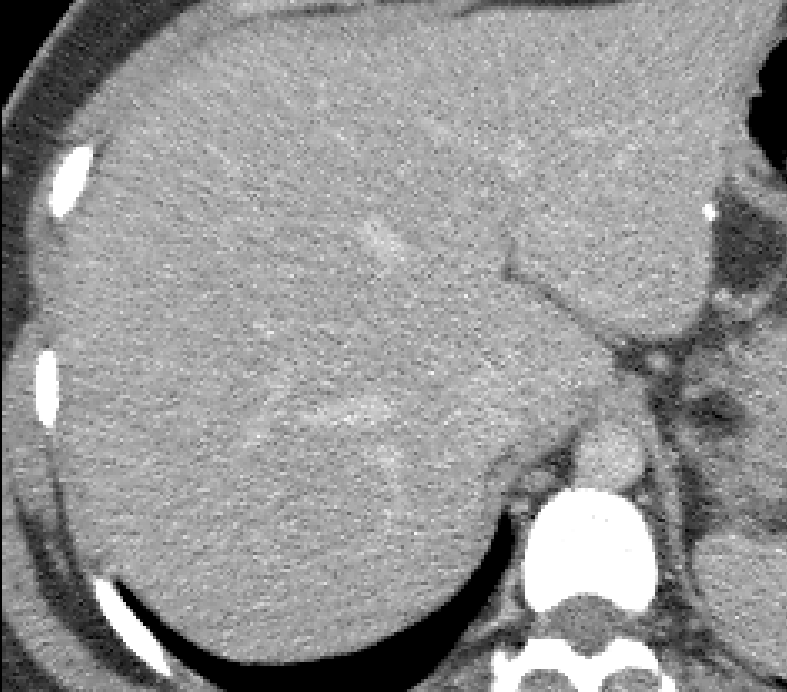
\includegraphics[height=4cm]{Images/noise_CT.png}
    \caption{Visualisation du bruit sur une image du foie. Celui-ci produit une texture sabloneuse.}
    \label{fig:CT_noise}
\end{figure}

Enfin, ce type d'imagerie est sensible à un troisième type d'artefacts lié aux objets métalliques tels que les broches. Ces objets provoquent des phénomènes de saturation sous formes de rayons concentriques visibles en Fig. \ref{fig:metallic artefacts}.

\begin{figure}
    \centering
    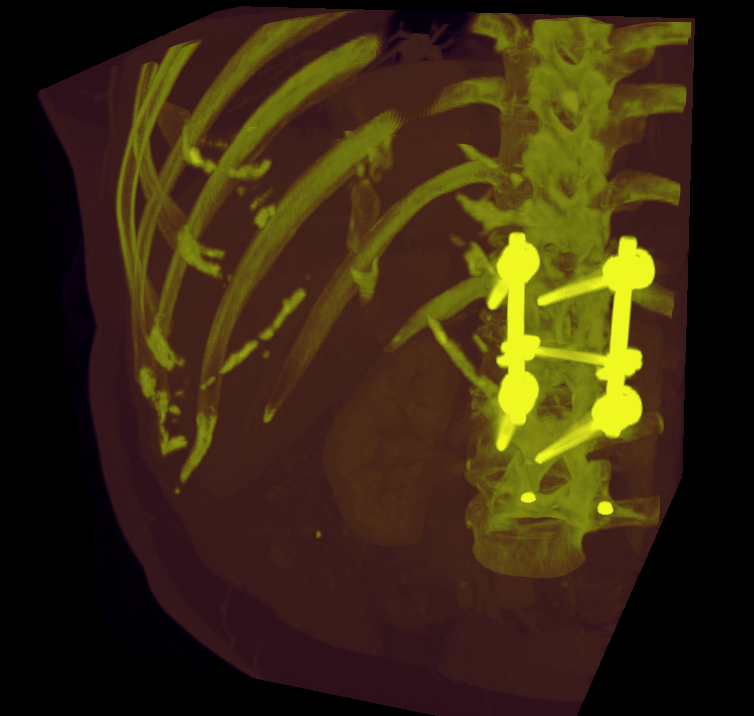
\includegraphics[height=4cm]{Images/broaches_CT.png}
    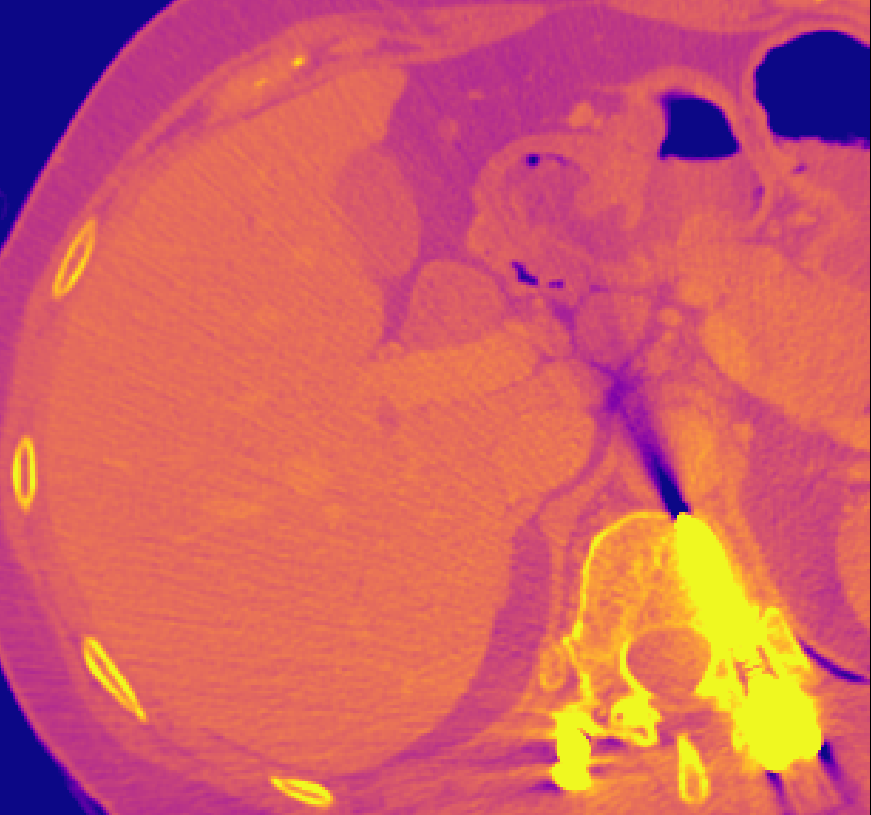
\includegraphics[height=4cm]{Images/broaches_CT_slice.png}
    \caption{Les broches métalliques visibles dans la vue 3D, provoquent des artefacts de saturation et de rayonnement visibles sur les vues en tranches.}
    \label{fig:metallic artefacts}
\end{figure}

Les intensités des images tomodensitométriques sont encodées dans une unité particulière, l'unité Houndfield (HU). Cette unité mesure le coefficient d'atténuation du rayonnement. Elle fixe à 0 l'atténuation de l'eau distillée et à $-1000$ l'atténuation de l'air. La limite haute dépend du nombre de bits utilisés pour l'encodage des pixels de l'image ($\sim 3071$ HU pour l'acier en 12 bits vs $\sim 13588$ HU en 16 bits) \cite{Glide2013_metal_saturation}. Cette gamme élevée de niveaux de gris n'est pas détectable dans son ensemble par l'oeil humain et nécessite des écrans spécifiques ou l'utilisation de fenêtres d'intensités ajustables dynamiquement.

L'acquisition des images se fait coupe par coupe. Pour obtenir une image en trois dimensions, il suffit d'empiler les coupes 2D.

\subsection{Imagerie par résonance magnétique}
\label{sec:contexte:images:irm}

Les premières images du corps humain obtenues par résonance magnétique (IRM) ont été réalisées par Damadian et al. en 1977 \cite{Damadian1977_NMRI}. Les machines utilisées pour l'imagerie par résonance magnétique sont similaires en apparence à la tomodensitométrie. Le patient est aussi allongé sur une table et est positionné à l'intérieur d'un anneau, Cependant, l'anneau contient des aimants qui produisent des champs magnétiques.

L'IRM repose sur la mesure du retour à l'équilibre du moment magnétique de particules chargées. Lorsque certains atomes sont soumis à un champ magnétique, ceux-ci s'orientent dans la direction du champ magnétique. Dans un système IRM, un champ magnétique constant permet d'aligner les atomes d'hydrogènes constitutifs des tissus dans une certaine direction appelée axe longitudinal. Ces particules sont en préhension, c'est-à-dire qu'elles tournent sur elles même autour de l'axe longitudinal comme une toupie qui se stabilise le long de son axe de rotation. Lors de l'acquisition, un deuxième champ magnétique orthogonal au premier champ magnétique provoque une résonance avec les atomes d'hydrogènes qui sont contraints d'augmenter leur angle de précession. Ce champ magnétique est ensuite arrêté, ce qui provoque un retour à la normale de la précession des atomes d'hydrogènes. C'est le temps que prend la précession pour se réaligner avec l'axe longitudinal, appelé temps de relaxation, qui est à la base de différentes mesures physiques permettant de produire différentes séquences d'images en IRM (Fig. \ref{fig:T1_MRI}).

Le temps de relaxation est dépendant de l'agitation moléculaire. Si l'agitation est très faible comme dans les tissus durs (os), ou très forte, la relaxation est lente. Au contraire, une agitation modérée, caractéristique des tissus mous produit une relaxation rapide.

\begin{figure}
    \centering
    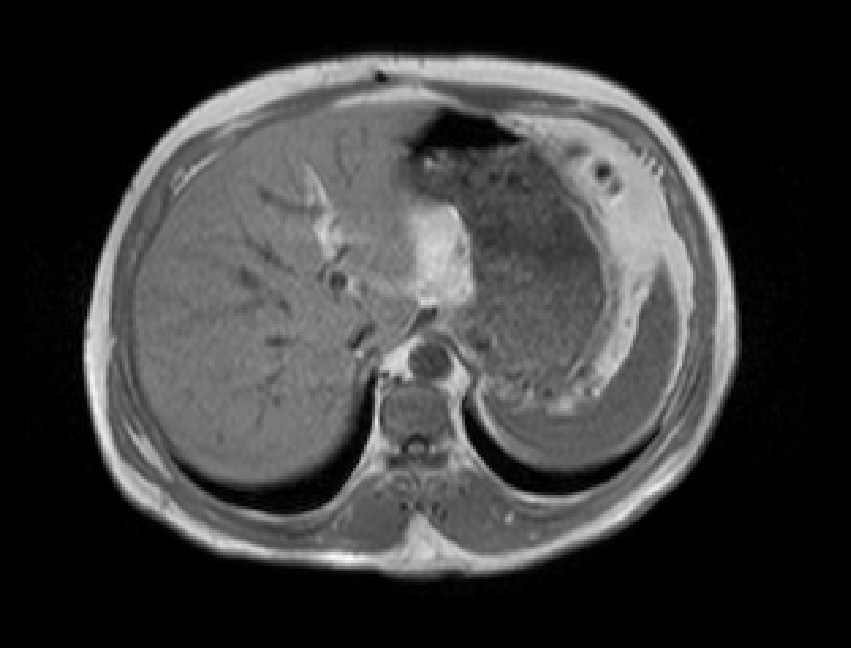
\includegraphics[height=4cm]{Images/T1_in_phase.png}
    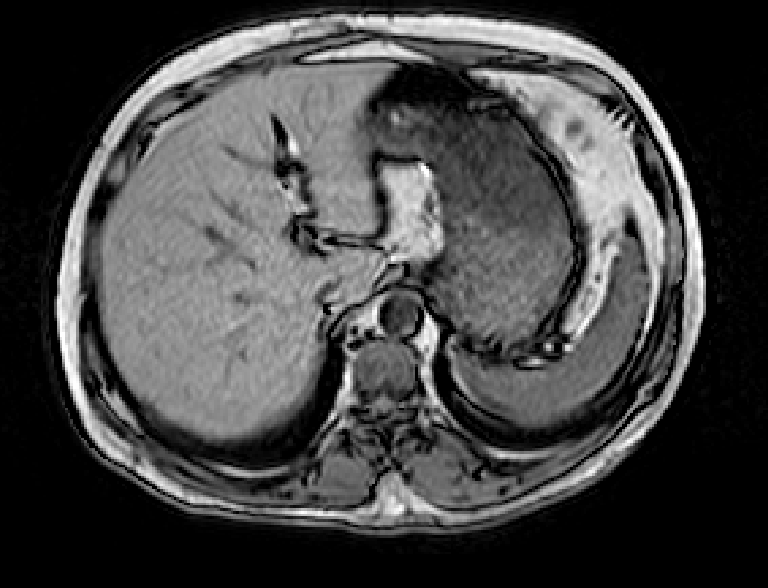
\includegraphics[height=4cm]{Images/T1_out_phase.png}
    \caption{Volumes de la base Chaos en phase T1-in (gauche) et T1-out (droite). La différence du temps d'écho entre l'émission et la réception du signal produit contrastes différents.}
    \label{fig:T1_MRI}
\end{figure}

\subsubsection{Artefacts des images IRM}

Les images IRM sont affectées par de nombreux artefacts. Nous présentons ici les trois principaux.

Premièrement, l'acquisition IRM dure environ 20 à 30 minutes. Il est demandé au patient de ne pas bouger durant l'acquisition et des acquisitions en apnées peuvent être nécessaires pour l'imagerie abdominale. Pour certains patients, cet exercice peut-être difficile voir douloureux à réaliser. Il est donc courant d'observer des artefacts liés au mouvement dans les images IRM (Fig. \ref{fig:MRI_movement}). Ceux-ci sont visibles de deux manières, la présence d'un organe fantôme légèrement décalé par rapport à l'organe lui-même ou la fusion des tissus d'organes adjacents. Deux organes peuvent aussi se superposer et une fusion des tissus peut être visible sur les images.

\begin{figure}
    \centering
    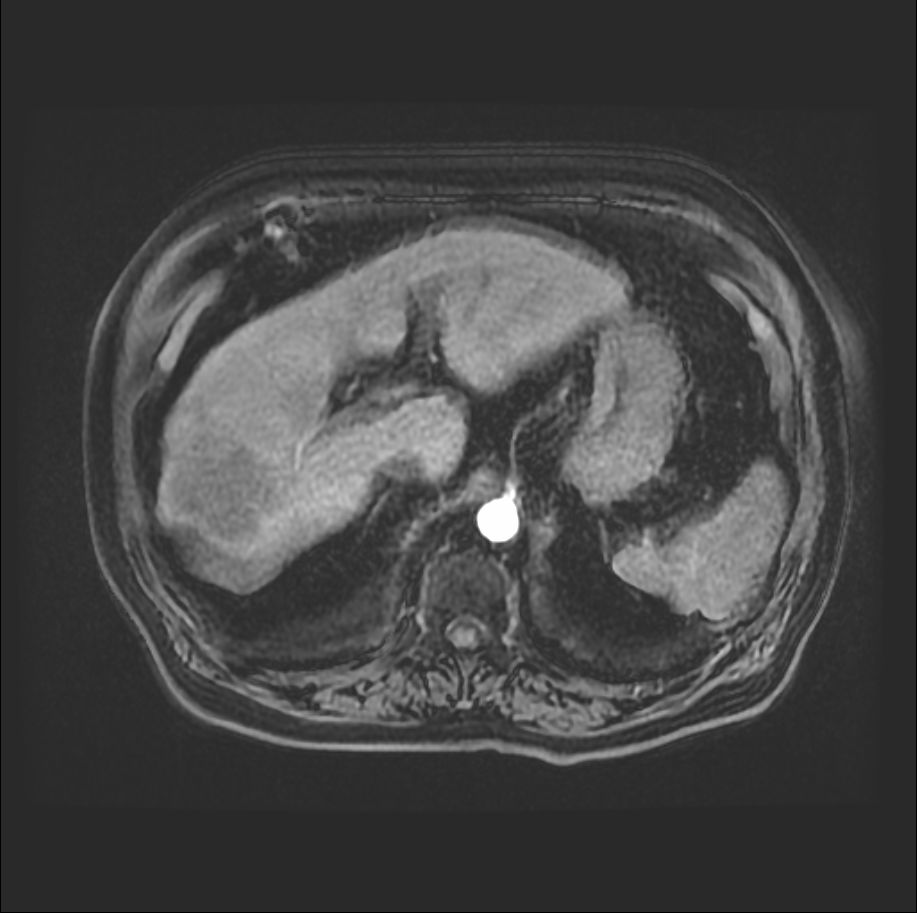
\includegraphics[height=5cm]{Images/MRI_movements.png}
    \caption{Artefacts de mouvement visibles sur les bordures du foie.}
    \label{fig:MRI_movement}
\end{figure}

Le bruit est aussi présent dans les images IRM, ce bruit est particulier puisqu'il s'agit d'un bruit ricien. Ce bruit n'est pas additif comme le bruit gaussien, mais est dépendant du signal. Il s'exprime par la densité de probabilité suivante : 

\begin{equation}
    f(x | \mu, \sigma) = \frac{x}{\sigma^2} exp ( (-x^2 + \mu^2)/(2\sigma^2) ) I_0 (\frac{x\mu}{\sigma^2})
    \end{equation}

Avec $I_0(z)$ la fonction de Bessel de première espèce et d'ordre 0. 

Lorsque le SNR est faible, la densité de probabilité de ce type de bruit ne suit pas du tout une densité de probabilité de bruit gaussien. Lorsque celui-ci augmente, la densité de probabilité approxime une distribution gaussienne (Fig. \ref{fig:MRI_Rice}).

\begin{figure}
    \centering
    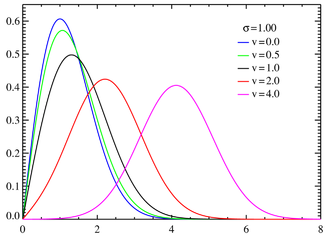
\includegraphics[height=4cm]{Images/rice_PDF.png}
    \caption{Distributions de Rice. Lorsque $\mu$ est faible, la partie gauche de la courbe présente une forte pente.}
    \label{fig:MRI_Rice}
\end{figure}

Le positionnement de l'antenne par rapport au corps du patient peut aussi entrainer des variations dans le champ magnétique qui provoquent des variations d'intensité locales dans des zones homogènes. Ainsi, des tissus de même nature peuvent montrer des profils d'intensité variés comme sur la Fig. \ref{fig:MRI_variations}.

\begin{figure}
    \centering
    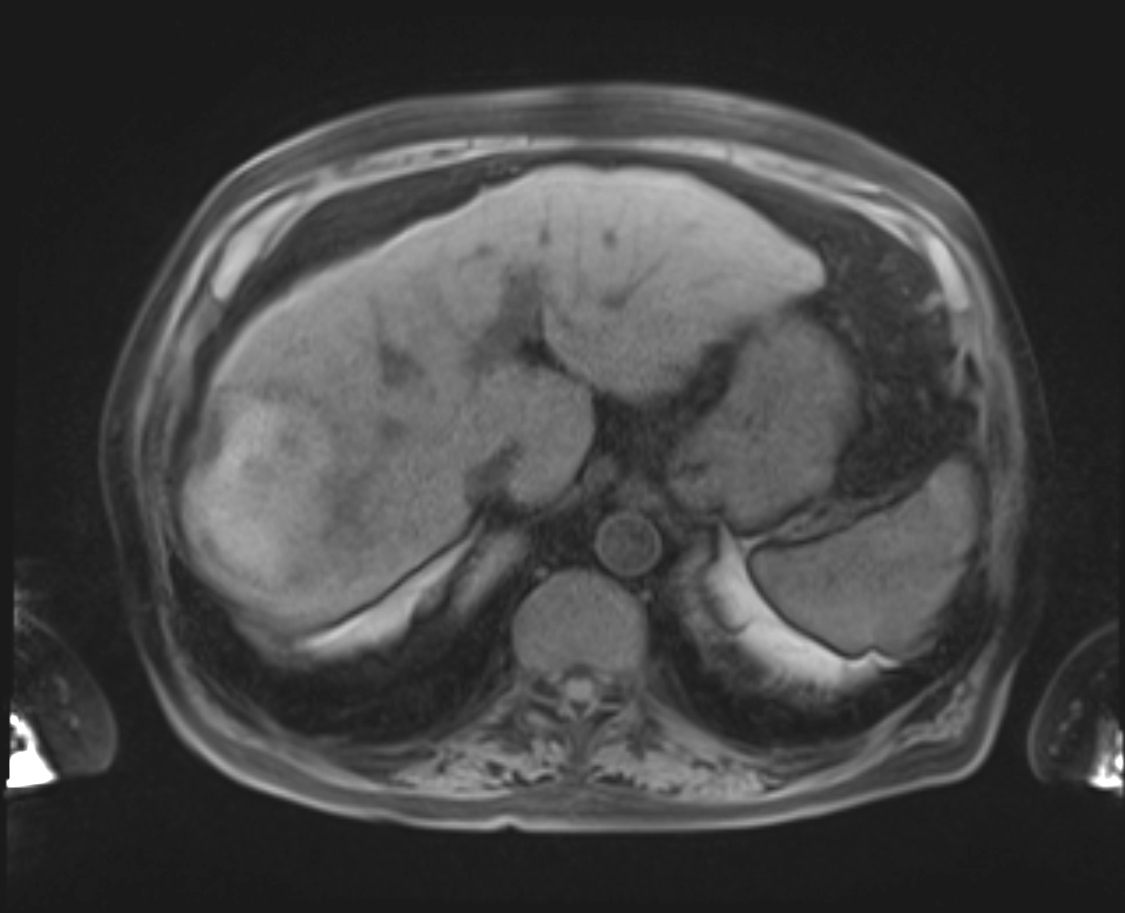
\includegraphics[height=4cm]{Images/MRI_field_variations.png}
    \caption{IRM du foie, T1-in. On observe une variation d'intensités pour des tissus de mêmes natures}
    \label{fig:MRI_variations}
\end{figure}

\section{Données}

L'annotation des données est une tâche complexe. Elle nécessite la supervision d'un médecin expert, car les organes à annoter sont complexes à identifier. Plusieurs types d'annotations sont possibles. Pour les vaisseaux sanguins par exemple, on peut choisir d'annoter la ligne centrale. On peut alors définir cette ligne comme une courbe passant par une série de points de contrôles. Cette méthode est économe en temps d'annotations, mais ne fournit généralement pas des informations précises sur l'aspect des vaisseaux et leurs diamètres. 
Une autre méthode consiste à créer un masque de segmentation en annotant les voxels appartenant aux vaisseaux. Cette méthode est la plus complète, mais nécessite bien plus de temps à l'annotateur. De plus, la notion de frontière entre les structures est subjective et varie d'un avis d'expert à l'autre. Une solution optimale est de moyenner le résultat parmi plusieurs annotateurs. Cette méthode demande cependant une mobilisation d'un nombre important de médecins. Il faut garder à l'esprit que dans un hôpital, un médecin peut rarement consacrer du temps pour annoter des données ce qui rend ce type d'initiatives rare.

Les deux types d'annotations sont illustrés en figure \ref{fig:annotations}. 

\begin{figure}
    \centering
    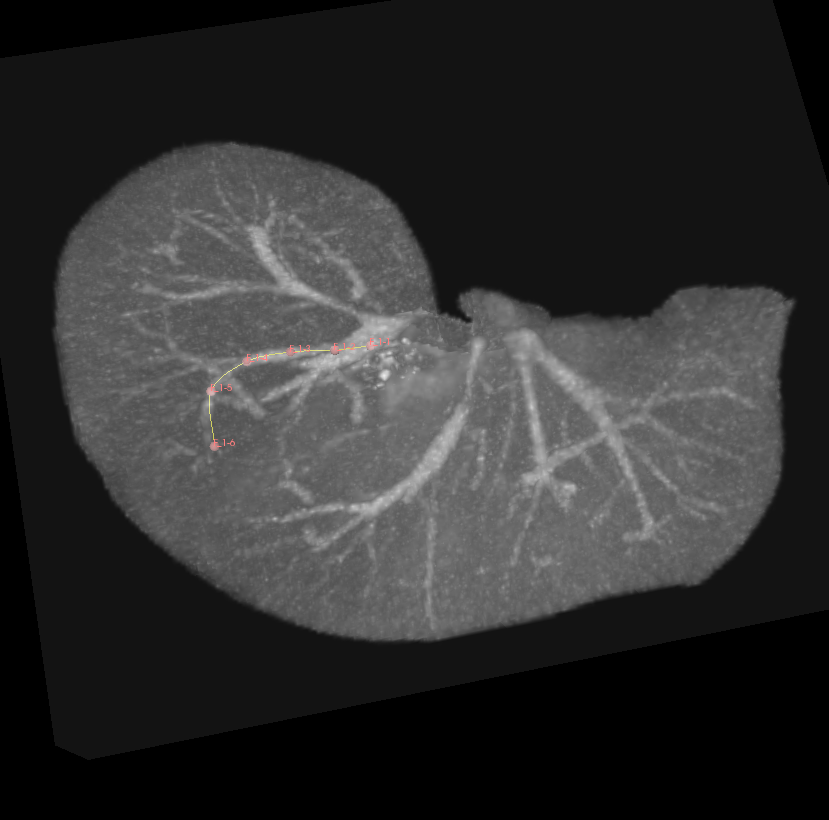
\includegraphics[height=4cm]{Images/centerline.png}
    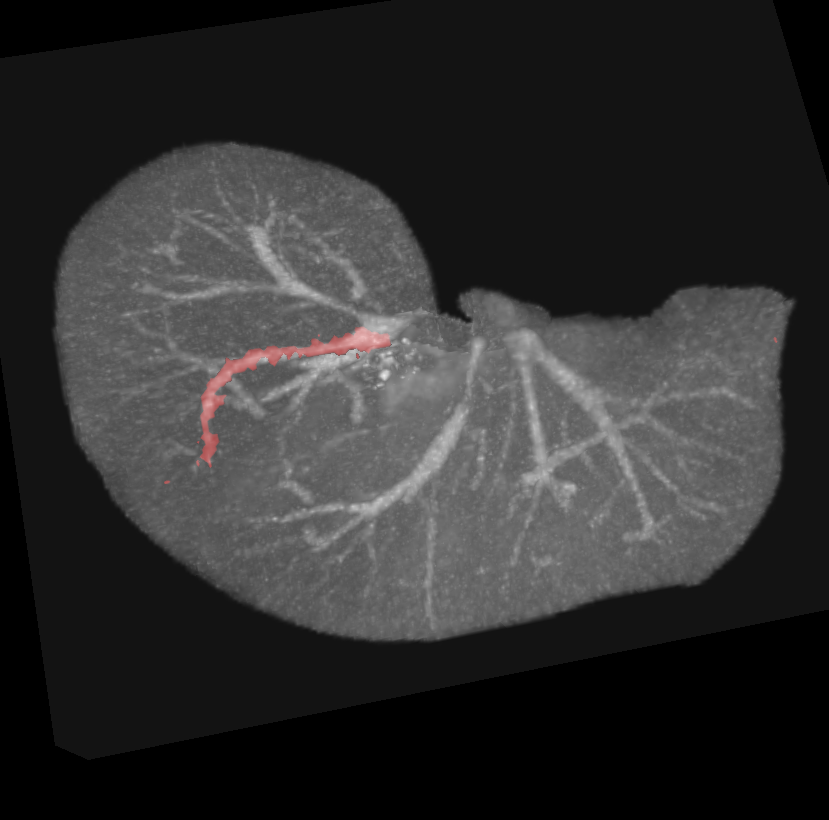
\includegraphics[height=4cm]{Images/segmentation.png}
    \caption{Annotations d'un vaisseau : ligne centrale vs masque de segmentation}
    \label{fig:annotations}
\end{figure}

De plus, l'accès aux données TDM et IRM peut-être difficile. La législation sur la protection des données personnelles puis la directive européenne complexifient l'accès aux données personnelles. En effet, la collecte de données dans un hôpital est soumise à un accord préalable d'un comité éthique puis de l'accord des patients. Pour la recherche, les données qui sont transmises doivent être anonymisées, c'est-à-dire que les informations contenues dans les images telles que le nom du patient, le nom de la série ainsi que la date de l'acquisition doivent être effacés. Cependant, depuis la mise en place de la RGPD, le patient a la possibilité de rétracter son avis à tout moment ce qui nécessite une politique d'anonymisation qui permette un suivi des données. On peut citer par exemple la \textit{tokenization}, qui permet d'attribuer une signature chiffrée à un volume.

Face à ces difficultés, une grande partie des bases des données utilisées dans les résultats de publications sont privées. L'auteur cite en général les conditions d'acquisition et le nombre de volumes disponibles, mais ne donne pas un accès aux données. Certains jeux de données sont tout de même disponibles publiquement. Nous passons ici en revue les jeux de données publique pour l'organe du foie et discutons des alternatives disponibles.

\subsection{Ircad}

La base de donnée 3DIrcadb1 est proposée par l'Institut de recherche contre les cancers de l'appareil digestif (Ircad) de Strasbourg. Cette base contient des images de tomodensitométrie de l'abdomen (Fig. \ref{fig:Ircad_examples}). Elle contient les images de 20 patients répartis en 50 \percent homme/femme et 75 \percent de foies lésés. Pour chaque patient une image tomographique inclut le foie et mesure entre $512 \times 512 \times 74$ et $512 \times 512 \times 260$ voxels pour une résolution des coupes axiales variant entre 0.56 mm et 0.87 mm et une épaisseur des coupes variant entre 1.00 mm et 4.00 mm. Elle fournit aussi un masque voxélique des organes de l'abdomen. Pour le foie, les masques des deux systèmes veineux porte et cave sont fournis dans des volumes différents. Un masque des tumeurs du foie est aussi disponible.

\begin{figure}
    \centering
    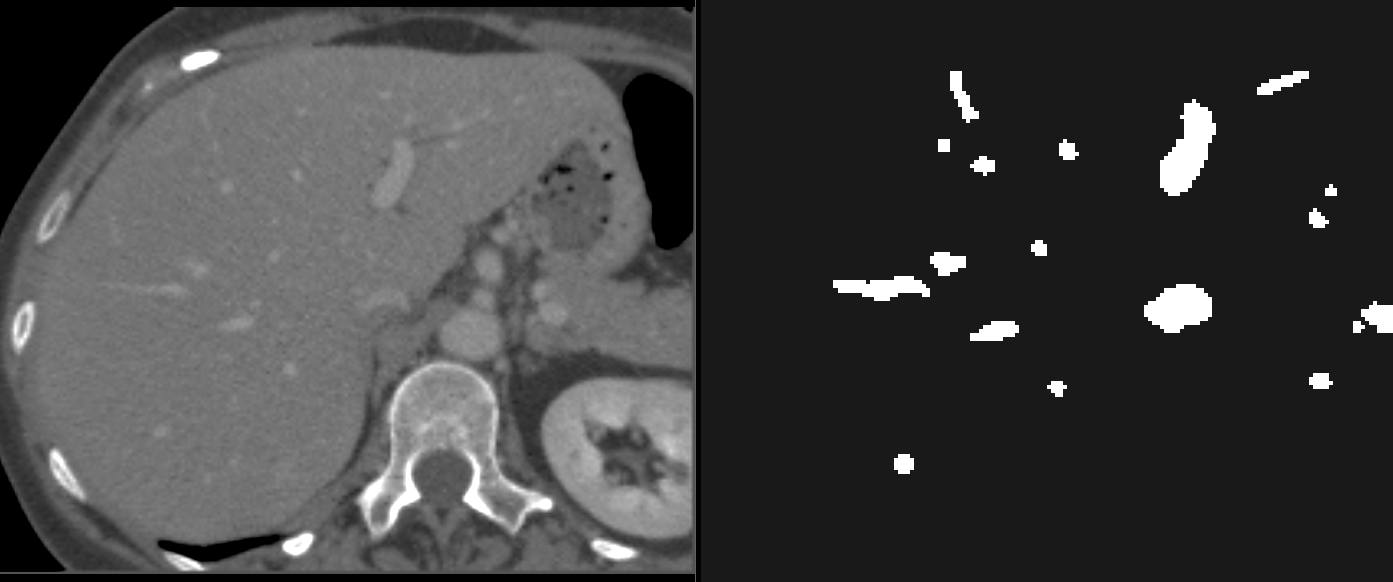
\includegraphics[height=5cm]{Images/Ircad_examples.png}
    \caption{À gauche, coupe du foie issue d'un volume de l'Ircad. À droite, vérité terrain des vaisseaux}
    \label{fig:Ircad_examples}
\end{figure}

Cette base datant de 2010 est la base la plus complète pour la segmentation des vaisseaux du foie. Cependant, elle n'est pas exempte d'anomalies. Premièrement, le nom des vérités terrain n'est pas consistant : le masque des veines portes est appelé "portal vein" quand celui de la veine cave est appelé soit "venous system" ou "vena cava". Cette différence de nom indique sans doutes que deux médecins différents ont participé à l'annotation des données. Deuxièmement, des voxels parasites sont présents dans le volume du masque du foie produisant des petites composantes connexes qui interfèrent avec les traitements sur les masques comme la sélection de la boîte englobante du foie. Enfin, certains vaisseaux à l'intérieur du foie ne sont pas annotés. Cela concerne des petites structures tubulaires mesurant quelques voxels de large, mais aussi de gros vaisseaux (Fig. \ref{fig:missing_annotations}). Ces oublis perturbent forcément l'évaluation des méthodes de segmentation puisque des vaisseaux non annotés pourraient tout de même être détectés et comptés comme des segmentations erronées. 

Ce biais est cependant appliqué à toutes les méthodes utilisant ces données ce qui en limite la portée dans les mesures de performances.
\todo{@Nicolas : Je veux bien les arguments de discussion ici, on avait abordé ce point il y a longtemps, c'est un peu loin...}

\begin{figure}
    \centering
    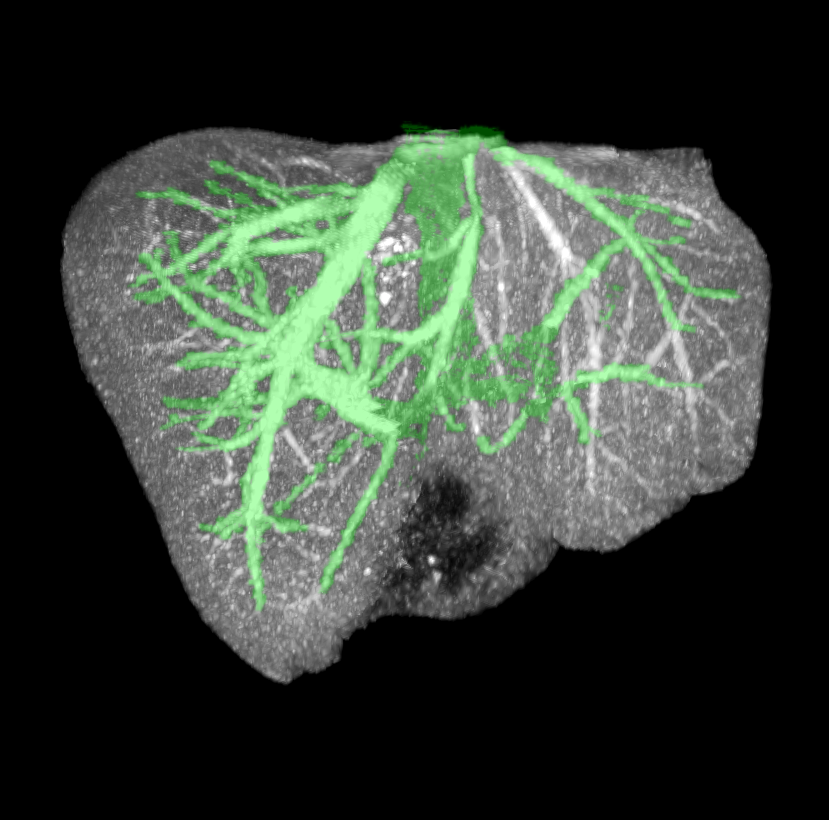
\includegraphics[height=5cm]{Images/missing_annotations.png}
    \caption{Vue 3D du foie. En vert, vérité terrain des vaisseaux. Des vaisseaux très visibles en 3D ne sont pas inclus dans la vérité terrain.}
    \label{fig:missing_annotations}
\end{figure}

\subsection{CHAOS}

Le jeu de donnée CHAOS est issu du challenge du même nom (CHAOS challenge - combined (CT-MR) Healthy Abdominal Organ Segmentation). Celui-ci propose deux jeux de données avec deux modalités différentes. Un premier jeu contient 40 images TDM obtenues après injection d'agent de contraste dans la veine porte. L'acquisition est prise 70-80 secondes après l'injection et elle permet de mettre en valeur le système veineux porte et une partie de la veine hépatique. Ce jeu de donné possède des images de résolution $512\times 512$ avec une résolution entre 0.7 mm et 0.8 mm dans le plan XY et 3 mm à 3.2 mm dans l'axe Z.

Un second jeu IRM inclut 120 volumes acquis selon des méthodes différentes : 40 volumes acquis en phase T1-in (Fig. \ref{fig:T1_MRI}), 40 volumes  en phase T1-out (Fig. \cite{fig:T1_MRI}) et 40 séquences en phase T2 spiralé (Fig. \ref{fig:T2_MRI}). La pondération de contraste T2 rend les vaisseaux du foie hyper-intense et l'acquisition spiralée permet de mieux séparer les tissus tout en limitant les artefacts de mouvement.

\begin{figure}
    \centering
    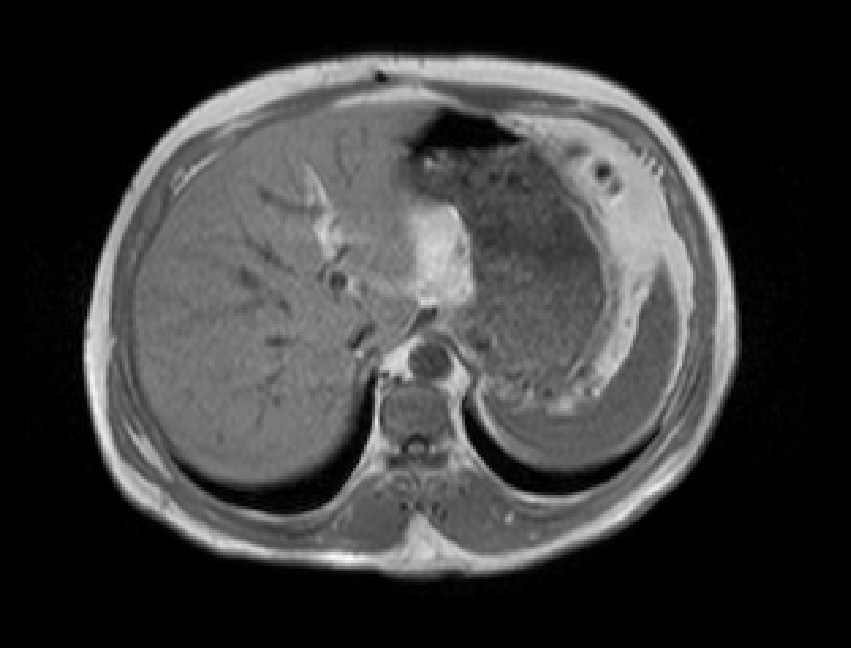
\includegraphics[height=4cm]{Images/T1_in_phase.png}
    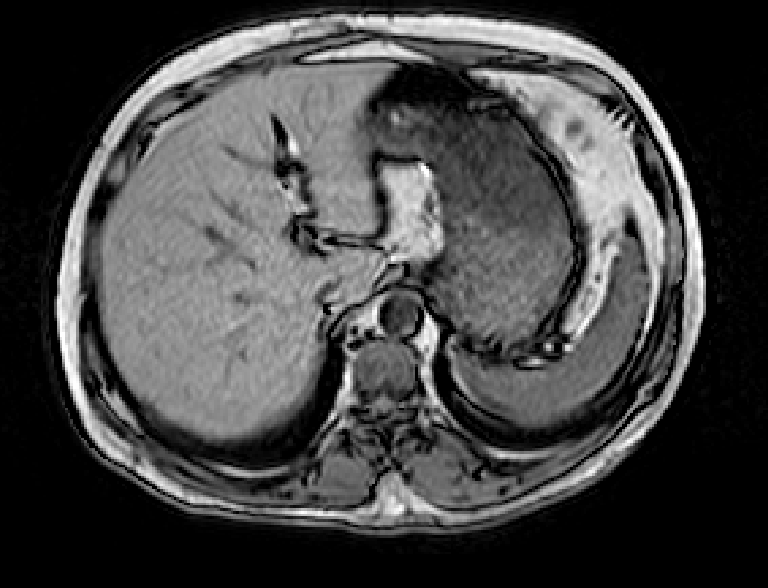
\includegraphics[height=4cm]{Images/T1_out_phase.png}
    \caption{Volumes de la base CHAOS en phase T1-in (gauche) et T1-out (droite). La différence du temps d'écho entre l'émission et la réception du signal produit contrastes différents.}
    \label{fig:T1_MRI}
\end{figure}

Cette base de donnée est complète dans le sens où elle propose deux modalités avec plusieurs modes d'acquisitions. Contrairement à l'Ircad, la résolution dans l'axe Z est plus élevée (Fig. \ref{fig:CHAOS_geometry}) ce qui indique que la base a été acquise en vue de traitements coupe par coupe plutôt que volumique. La page d'information du Grand Challenge abonde d'ailleurs en ce sens en précisant le nombre de coupes totales ainsi que leur répartition en jeu d'entrainement et de test. De plus, l'objectif de cette base étant la segmentation des organes abdominaux, elle ne propose que le masque du foie comme annotation.

\begin{figure}
    \centering
    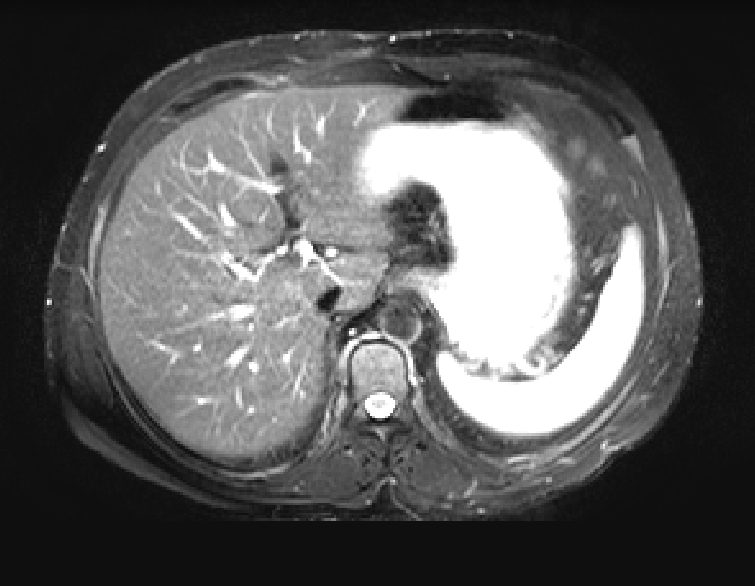
\includegraphics[height=4cm]{Images/T2_SPIR.png}
    \caption{Volumes de la base CHAOS acquise en phase T2 spiralée. Le contraste des vaisseaux est plus important en pondération T2.}
    \label{fig:T2_MRI}
\end{figure}

\begin{figure}
    \centering
    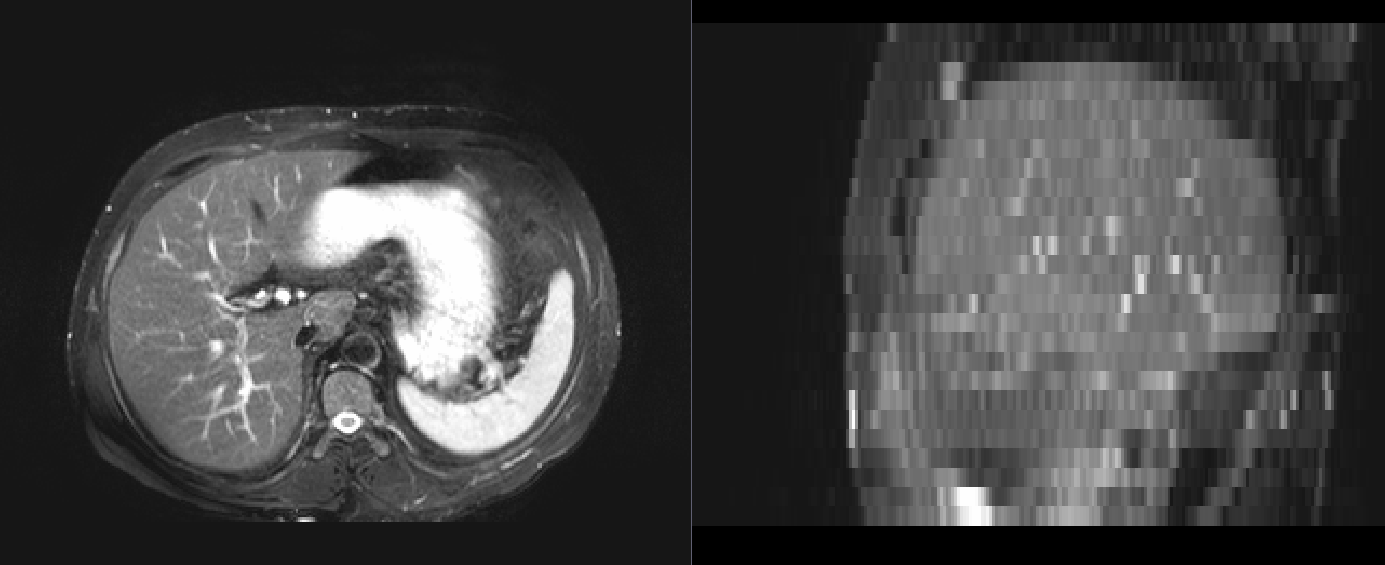
\includegraphics[height=4cm]{Images/CHAOS_resolution.png}
    \caption{comparaison de la résolution axial (gauche) et sagitale (droite). Dans la vue sagitale la géométrie des structures est largement altérée.}
    \label{fig:CHAOS_geometry}
\end{figure}

\subsection{Medical Decathlon}

Le Challenge Medical Decathlon propose de mesurer les performances d'algorithmes de segmentations sur 10 tâches qui regroupent différents organes (cerveau, cœur, hippocampe, foie, pancréas, prostate, colon, rate). Le Challenge regroupe un nombre significatif de volumes par tâches, de 30 volumes pour le cœur jusqu'à 750 volumes pour le cerveau. Une modalité par organe est proposé : IRM pour le cerveau, le cœur, l'hippocampe, la prostate et la tomodensitométrie pour les autres organes. Deux tâches concernent le foie, toutes deux acquises en phase veineuse porte. La première tâche concernant la segmentation du foie et des tumeurs hépatiques contient 210 volumes. La seconde tâche concernant la segmentation des vaisseaux et des tumeurs hépatiques regroupe 443 volumes.

Les données hépatiques pour la première tâche ont été sélectionnées pour leur variabilité en termes de taille de labels avec de fortes variations de tailles de foie, de nombre de tumeurs, etc. Ces données ont été acquises au centre de l'Ircad de Strasbourg. La résolution des images pour cette tâche est de 0.5 mm à 1.0 mm dans l'axe XY et 0.45 mm à 6.0 mm dans l'axe Z. Les annotations sont faites par un expert radiologue.

Les données hépatiques pour la seconde tâche (Fig. \ref{fig:MD_examples}) sont issues de patients présentant des tumeurs hépatiques parfois métastasés. Les vaisseaux sanguins présentent parfois des connexions au niveau des tumeurs. Ces données ont été acquises par le centre contre le cancer Memorial Sloan à New York. Pour cette tâche, la résolution des images dans l'axe Z varie de 2.5 mm à 5.0 mm. Les masques de segmentation ont été annotés de manière semi-automatique par une approche par croissance de région. Les contours ont ensuite été ajustés par des radiologues.

Cette base de données à l'avantage de proposer un grand nombre de volumes dans plusieurs modalités. Cependant, l'annotation semi-automatique produit une vérité terrain moins précise, en particulier pour les petits vaisseaux. On peut aussi noter un nombre conséquent de vaisseaux déconnectés du réseau vasculaire dans les annotations. De plus, pour le foie, les pas supérieurs à 3 mm dégradent fortement la géométrie des vaisseaux lorsque l'on considère une approche de segmentation/détection 3D, comme illustrée dans CHAOS (Fig. \ref{fig:CHAOS_geometry}).

\begin{figure}
    \centering
    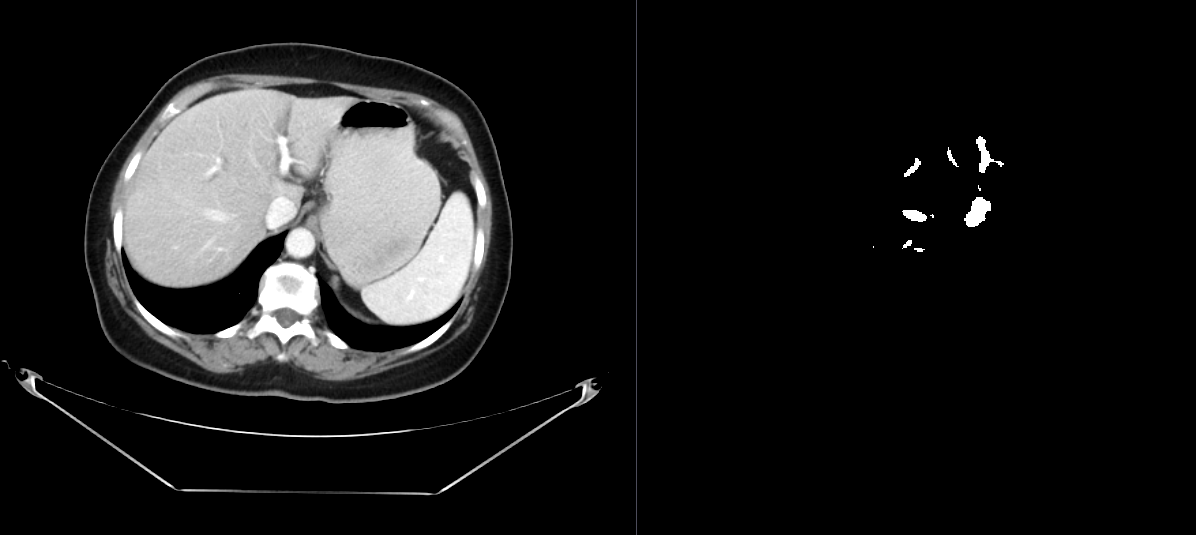
\includegraphics[height=4cm]{Images/MD_examples.png}
    \caption{Challenge Médical Décathlon. Volumes TM hépatique (gauche) et la vérité terrain associée.}
    \label{fig:MD_examples}
\end{figure}

\subsection{Données synthétiques : VascuSynth}

Lorsque des données cliniques avec des annotations sont difficiles à obtenir, une autre solution est de générer un volume contenant un réseau vasculaire synthétique. VascuSynth est un programme permettant de créer un réseau vasculaire en fonction d'une carte d'oxygénation et des paramètres de pression sanguine à l'entrée de celui-ci. Le réseau vasculaire est construit de manière itérative de sa racine jusqu'aux extrémités. L'utilisateur peut de plus paramétrer la complexité du réseau en spécifiant le nombre de bifurcations attendues. Il est aussi possible d'ajouter du bruit additif gaussien au volume.

La résolution des volumes est  normalisée à 1 mm pour l'ensemble des axes. Les vaisseaux de VascuSynth présentent des profils d'intensité quasi homogènes, avec une intensité des voxels moindres près des bordures. Les volumes ont un fond nul. La vérité terrain des vaisseaux, précise au pixel près, peut donc être obtenue par simple seuillage.

Une base de donnée pré-générée est disponible sur le site de VascuSynth. Celle-ci propose 120 volumes répartis en 10 groupes de 12 volumes. Chaque groupe contient des volumes de réseaux vasculaires dont le nombre de bifurcations varie entre 1 et 56 avec un pas de 5 (1,6,11,...,56) comme illustré en Fig. \ref{fig:VascuSynth}. Le jeu de données est aussi fourni avec un fichier Matlab décrivant les coordonnées des bifurcations.

Les bases de données synthétiques possèdent les vérités terrain les plus complètes. Cependant, le contexte de ces jeux de données est beaucoup plus simple que les images réelles. Il est en effet difficile de simuler de manière réaliste des organes vascularisés dont les conditions de développement sont multifactoriels et qui dépendent à la fois de mécanismes génétiques et aléatoires qui sont en partie compris. Les vaisseaux générés sont ainsi plus simples, dans le cas de VascuSynth, les vaisseaux sont des tubes pleins droits discrétisés.

\begin{figure}
    \centering
    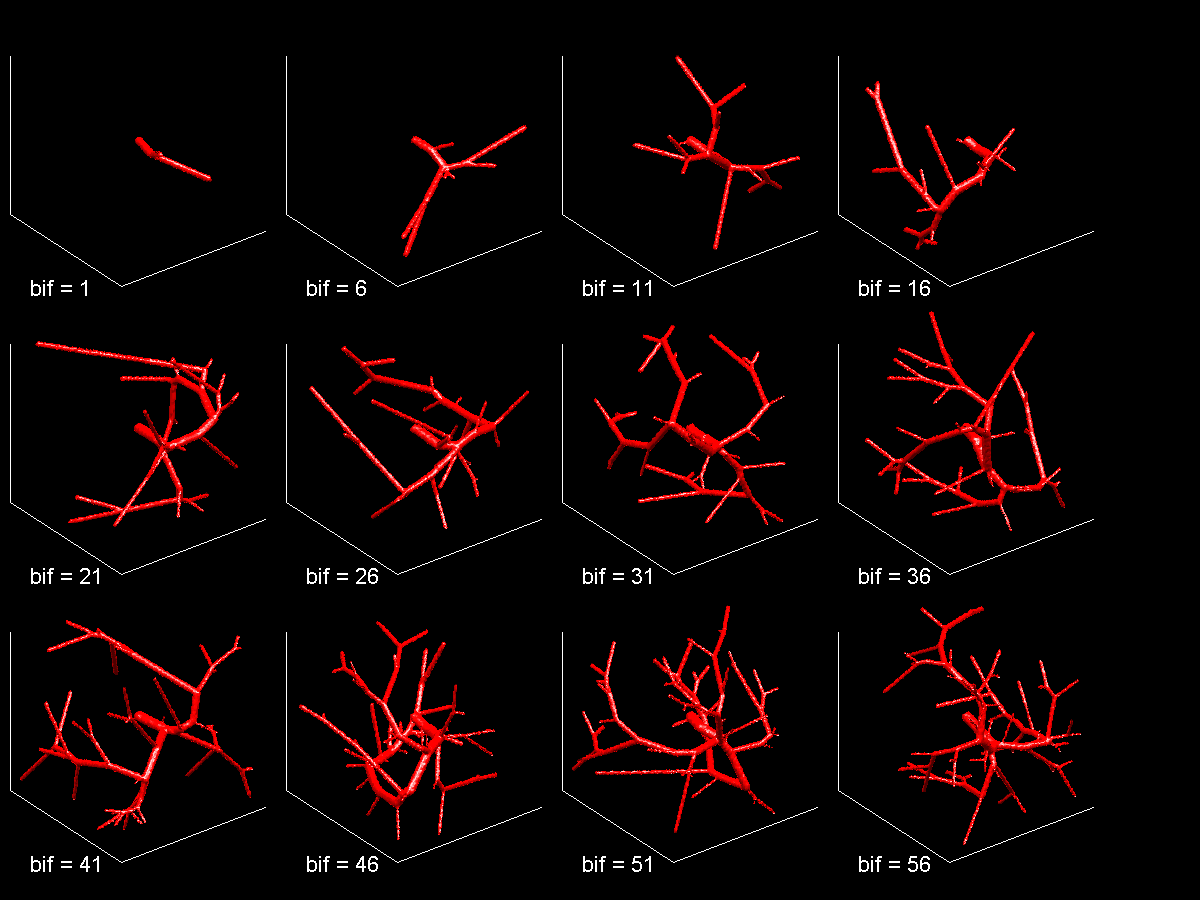
\includegraphics[height=4cm]{Images/snapVascu.png}
    \caption{Exemples de volumes issus de la base VascuSynth\_2013.}
    \label{fig:VascuSynth}
\end{figure}

\subsection{Bullitt}

Plus généralement, trouver des bases de données publiques d'images réelles vasculaires avec leur vérité terrain n'est pas simple. La base de donnée Bullitt est un jeu de données d'acquisitions IRM du cerveau. Sur une partie de ces données (une trentaine de volumes), la ligne centrale et le rayon des vaisseaux est fourni. Une segmentation des vaisseaux peut être reconstruite grâce à l'outil tubeTK ; cependant la reconstruction est faite à partir d'un tube circulaire et a tendance à sous-estimer / manquer des voxels appartenant aux vaisseaux.

Les travaux de Sanchesa et al. \cite{Sanchesa2019_annotations_deep} améliorent ces vérités terrains de manière significative en augmentant de 200 \percent le nombre de voxels appartenant à la segmentation initiale, ce qui permet l'utilisation d'annotations plus précises (Fig.  \ref{fig:Bullitt_annotation_ameliorations}).

\begin{figure}
    \centering
    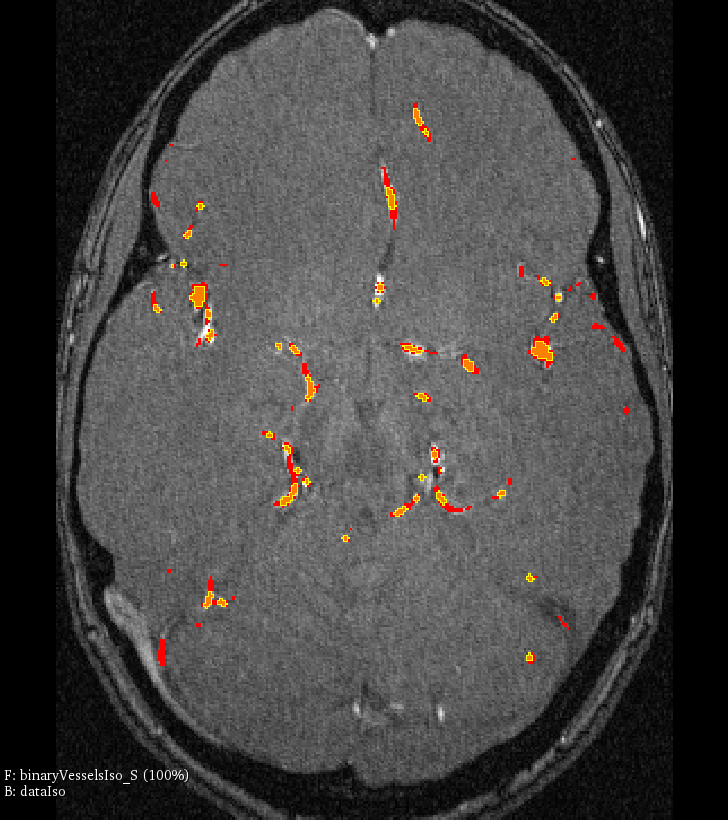
\includegraphics[height=4cm]{Images/Bullitt_annotation_ameliorations.png}
    \caption{Différence d'annotations entre reconstruction de la ligne centrale par tubeTK (jaune) et corrections d'annotations par (rouge). }
    \label{fig:Bullitt_annotation_ameliorations}
\end{figure}

Cette base de données est particulièrement bien acquise et présente très peu d'artefacts comparés à des images IRM classiques. Le seul artefact notable est un faible bruit constant sur l'ensemble de l'image (\ref{fig:Bullitt_example}).

\begin{figure}
    \centering
    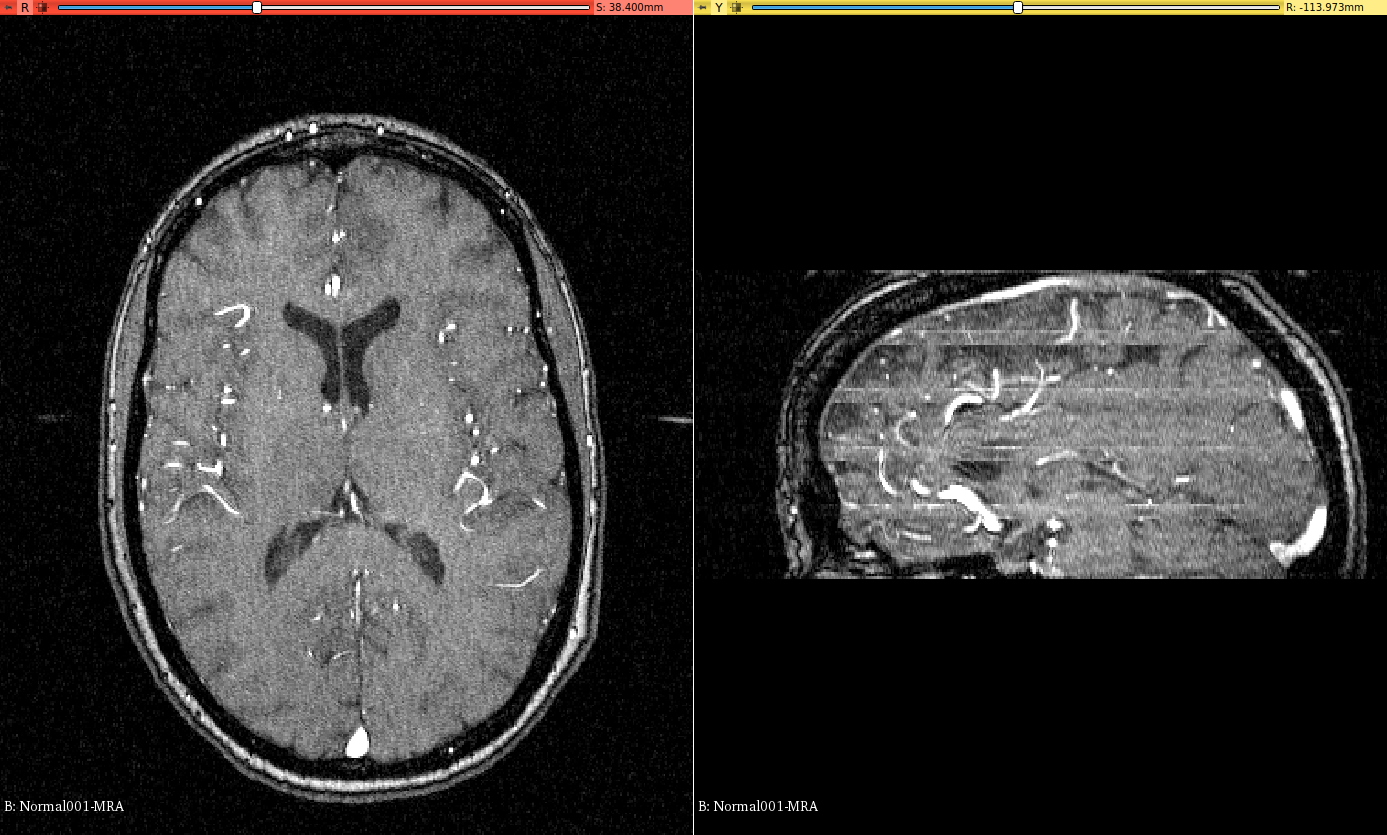
\includegraphics[height=4cm]{Images/Bullitt_examples.png}
    \caption{Exemples de volumes issus de Bullitt.}
    \label{fig:Bullitt_example}
\end{figure}


\subsection{Bases de données relatives au projet R-Vessel-X}

Il était prévu pour le projet ANR une campagne de collecte de données TDM et IRM durant la durée du projet et commençant en même temps que la thèse. Cette collecte devait être réalisée sur des patients en cours de traitement. Cependant, la nécessité d'obtenir un accord d'une commission éthique puis le besoin d'obtenir un espace de stockage dédié avec une société accréditée a retardé la collecte des données d'au moins un an. Celle-ci a finalement débouché sur une collecte de données rétrospective (patients ayant quitté l'hôpital) en même temps que le développement d'un logiciel d'annotations de données (voir Chap. 5). Ces données n'ont pas été exploitée dans nos travaux, puisqu’elles n’étaient pas prêtes au moment de notre étude.

\section{Bilan}

Dans un premier temps, nous avons choisi d'utiliser deux jeux de données : La base de l'Ircad et le jeu de données de VascuSynth\_2013. La base de l'Ircad contient des artefacts variés de TDM (bruit, artefacts métalliques, etc.) et des masques de segmentation pour tous les volumes. Cela nous permet d'évaluer plus aisément les performances des algorithmes employés dans nos travaux. De plus la résolution spatiale des volumes est une des meilleures parmi les bases disponibles. On peut ainsi utiliser des traitements 3D plutôt que de considérer un volume comme une séquence de coupes 2D. VascuSynth\_2013 offre une précision des vérités terrains qui n'est pas possible sur les bases réelles. C'est donc une base que nous avons jugé nécessaire pour notre travail. Celle-ci nécessite tout de fois un traitement complémentaire afin de rendre les volumes proches d'une acquisition réelle. Ce traitement est décrit dans le chapitre 3 où nous avons choisi d'ajouter des artefacts IRM aux données.

Afin de compléter nos jeux de données et diversifier nos expériences, nous avons ajouté la base de Bullitt pour ajouter des données réelles avec la modalité IRM. Un soin particulier a été apporté à l'acquisition des images pour Bullitt qui présente un contraste remarquable entre les vaisseaux et le reste de l'image. Ces conditions ne sont toutefois pas représentatives des images obtenues dans des examens classiques nous avons donc dégradé ces images.

Les qualités des trois bases de données sont récapitulées dans la Tab. \ref{tab:db_for_exp}.

\begin{table}
    \centering
    \begin{tabular}{ c|c|c }
        \hline
        Jeux de données & Modalités & Organe \\
        \hline
        Ircad           & TM & Foie \\
        VascuSynth      & Synthétique / IRM simulé & Aucun \\
        Bullitt         & IRM + artefacts ajoutés & Cerveau \\
        \hline
    \end{tabular}
    \caption{Bases de données retenues pour la suite de nos travaux.}
    \label{tab:db_for_exp}
  \end{table}


